\documentclass[a4paper, 11pt]{article}
\usepackage{comment} % enables the use of multi-line comments (\ifx \fi) 
\usepackage{lipsum} %This package just generates Lorem Ipsum filler text. 
\usepackage{fullpage} % changes the margin
\usepackage{graphicx}
\usepackage{epsfig}
\usepackage{listings}
\usepackage{xcolor}
\lstset { %
	language=C++,
	backgroundcolor=\color{black!5}, % set backgroundcolor
	basicstyle=\footnotesize,% basic font setting
}

\begin{document}
%Header-Make sure you update this information!!!!
\noindent
\large\textbf{Lab 3 Report} \hfill \textbf{Abhishek Srivastava} \\
\normalsize CS260-001: Computer Security \hfill Student Id: 861307778 \\
\normalsize Prof. Heng Yin \hfill \today \\
\hrule

\section*{Problem : Experimenting with Dynamic Taint Analysis in DECAF}
Objective for this lab assignment is to implement a register callback which can show us if EIP is tainted or not in case of buffer overflow.

\section*{Solution}
After following the instruction provided I created executable , start the windows system using DECAF and copying the ex01.exe to the windows system. After that I implemented the callback which will call in case of EIP is tainted in case.\\

In Figure 1 you can see the Keyboard input after loading the keylogger.so file. The ex01.exe is able to receive the keyboard inputed values from the qemu.\\

In the Figure 2 you can see that the program crashed due to the buffer overflow input.\\

Figure 3 shows the log of the only ex01.exe process. I am storing Tainted status of the program, Source\_eip address, Target\_eip address and Target\_eip\_taint value.\\

Figure 4 shows that I tested the program with taint pointers enabled as well but the result was the same as taint pointers off.\\
\newpage  
\begin{figure}
	\centering
	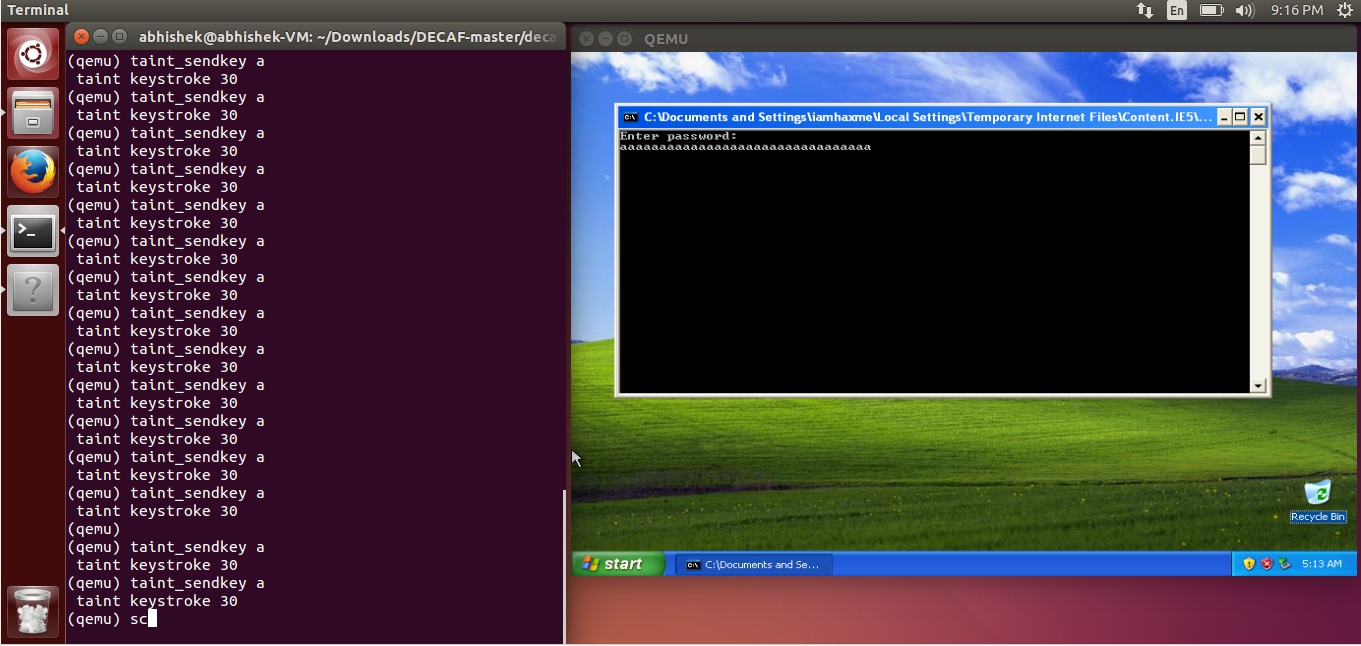
\epsfig{file=Lab_3_ss_1.png, height=3in, width=6in}
	\caption{Screen Shot of taint\_sendkey inputs to the ex01.exe .}
\end{figure}
\begin{figure}
	\centering
	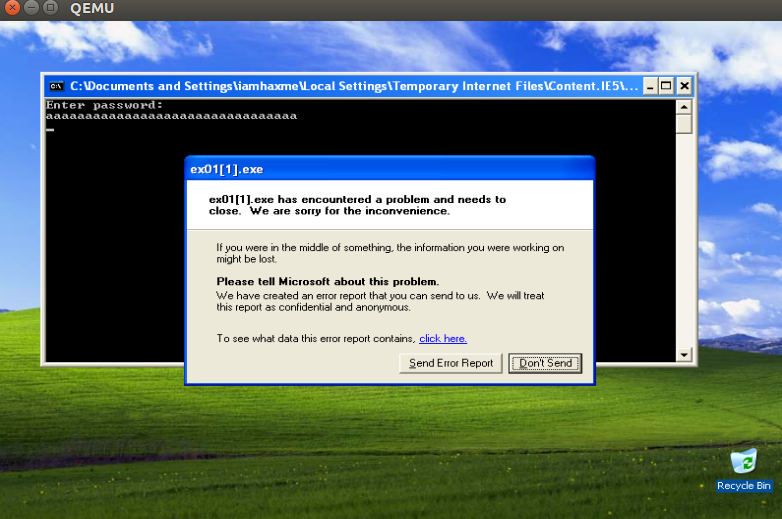
\epsfig{file=Lab_3_ss_2.png, height=4in, width=6in}
	\caption{Program Crashed for buffer overflow input.}
\end{figure}
\begin{figure}
	\centering
	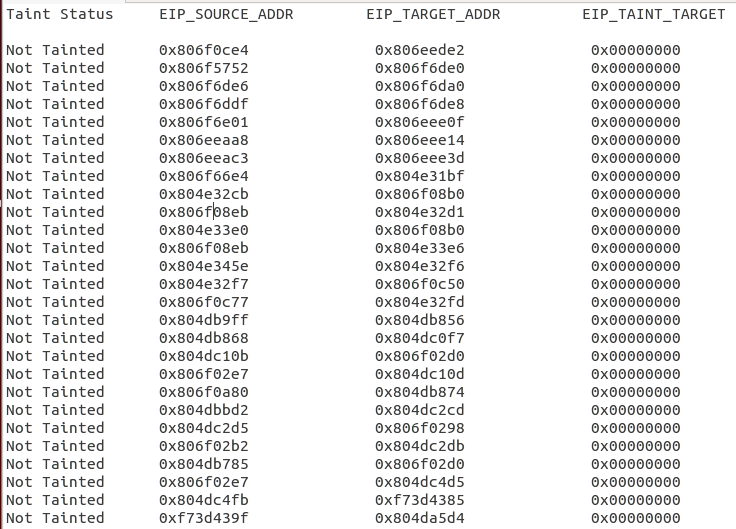
\epsfig{file=Lab_3_ss_3.png, height=5in, width=7in}
	\caption{Log values stored.}
\end{figure}
\begin{figure}
	\centering
	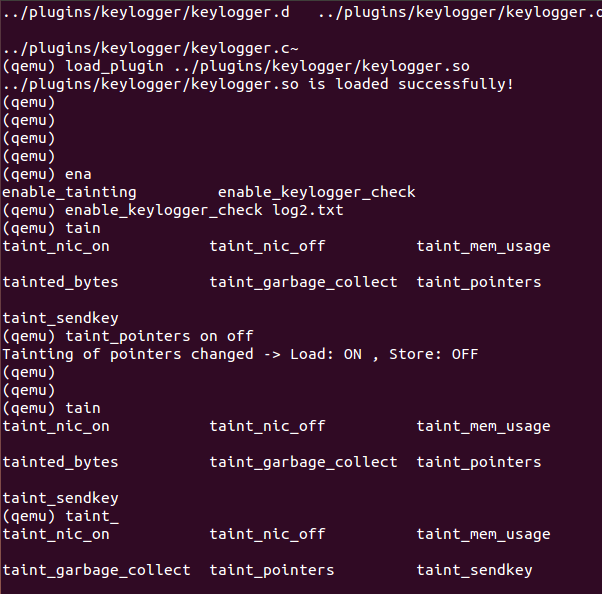
\epsfig{file=Lab_3_ss_4.png, height=6in, width=7in}
	\caption{Test after enabling the pointer tainting ON.}
\end{figure}

\newpage
\section*{Code Implementation of Callback}
\begin{lstlisting}
#include <sys/time.h>
#include <string.h>

#include "DECAF_types.h"
#include "DECAF_main.h"
#include "DECAF_target.h"
#include "hookapi.h"
#include "DECAF_callback.h"

#include "utils/Output.h"
#include "function_map.h"
#include "vmi_callback.h"
#include "vmi_c_wrapper.h"
//basic stub for plugins
static plugin_interface_t keylogger_interface;
static int taint_key_enabled=0;

DECAF_Handle keystroke_cb_handle = DECAF_NULL_HANDLE;
DECAF_Handle handle_write_taint_mem = DECAF_NULL_HANDLE;
DECAF_Handle handle_read_taint_mem = DECAF_NULL_HANDLE;
DECAF_Handle handle_block_end_cb = DECAF_NULL_HANDLE;
//for tainted EIP
DECAF_Handle eip_check_handler = DECAF_NULL_HANDLE;
FILE * keylogger_log=DECAF_NULL_HANDLE;
.
.
.

void my_eip_check(DECAF_Callback_Params *p) {
    
    uint32_t eip= DECAF_getPC(cpu_single_env);
    uint32_t cr3= DECAF_getPGD(cpu_single_env);
    char name[128];
    tmodinfo_t  dm;// (tmodinfo_t *) malloc(sizeof(tmodinfo_t));
    if(VMI_locate_module_c(eip,cr3, name, &dm) == -1)
    {
        strcpy(name, "<None>");
        bzero(&dm, sizeof(dm));
    }
    char* proc_name = "ex01.exe";
    int cmp_val = strcmp(name,proc_name);
    if(!cmp_val) {
        if(p->ec.target_eip_taint > 0) {
        printf("tainted\n ");
        fprintf(keylogger_log,"%s   \t 0x%08x \t\t 0x%08x \t\t 0x%08x\n", 
        "Tainted", 
        p->ec.source_eip, p->ec.target_eip, p->ec.target_eip_taint);
    } else
        fprintf(keylogger_log,"%s   \t 0x%08x \t\t 0x%08x \t\t 0x%08x\n",
        ``Not Tainted'', 
        p->ec.source_eip, p->ec.target_eip, p->ec.target_eip_taint);
    }
}
.
.
.
.
.
void keylogger_cleanup()
{
    if(keylogger_log)
    fclose(keylogger_log);
    if(handle_read_taint_mem)
        DECAF_unregister_callback(DECAF_READ_TAINTMEM_CB,handle_read_taint_mem);
    if(handle_write_taint_mem)
        DECAF_unregister_callback(DECAF_WRITE_TAINTMEM_CB,handle_write_taint_mem);
    //unregsitering        
    if(eip_check_handler)
        DECAF_unregister_callback(DECAF_EIP_CHECK_CB,my_eip_check);
    if(handle_block_end_cb)
        DECAF_unregisterOptimizedBlockEndCallback(handle_block_end_cb);
    handle_read_taint_mem = DECAF_NULL_HANDLE;
    handle_write_taint_mem = DECAF_NULL_HANDLE;
    keylogger_log = NULL;
    handle_block_end_cb = DECAF_NULL_HANDLE;
}

void do_enable_keylogger_check( Monitor *mon, const QDict *qdict)
{
    const char *tracefile_t = qdict_get_str(qdict, "tracefile");
    keylogger_log= fopen(tracefile_t,"w");
    if(!keylogger_log)
    {
        DECAF_printf("the %s can not be open or created !!",tracefile_t);
        return;
    }
    fprintf(keylogger_log,``TaintStatus    \t EIP_SOURCE_ADDR   
	    \t EIP_TARGET_ADDR \t EIP_TAINT_TARGET\n'');
    if(!handle_read_taint_mem)
        handle_read_taint_mem = DECAF_register_callback(DECAF_READ_TAINTMEM_CB,
        do_read_taint_mem,NULL);
    if(!handle_write_taint_mem)
        handle_write_taint_mem = DECAF_register_callback(DECAF_WRITE_TAINTMEM_CB,
        do_write_taint_mem,NULL);
    //registering
    if(!eip_check_handler)
        eip_check_handler = DECAF_register_callback(DECAF_EIP_CHECK_CB,
        my_eip_check,NULL);
    if(!handle_block_end_cb)
        handle_block_end_cb =  DECAF_registerOptimizedBlockEndCallback(
        do_block_end_cb, NULL, INV_ADDR, INV_ADDR);

}
.
.
static mon_cmd_t keylogger_term_cmds[] = {
#include "plugin_cmds.h"
{ NULL, NULL, }, };

plugin_interface_t* init_plugin(void) {
keylogger_interface.mon_cmds = keylogger_term_cmds;
keylogger_interface.plugin_cleanup = &keylogger_cleanup;

//initialize the plugin

return (&keylogger_interface);
}
\end{lstlisting}
\end{document}
